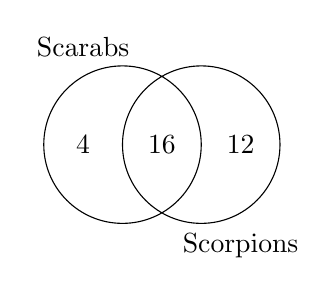
\begin{tikzpicture}
\draw(0,0)circle(1)(1,0)circle(1)(-0.5,0)node{$4$}(0.5,0)node{$16$}(1.5,0)node{$12$};
\draw(-.5,1)node[anchor=south]{Scarabs}(1.5,-1)node[anchor=north]{Scorpions};
\end{tikzpicture}

The diagram above shows the distribution of students in a $40$ person
desert ecology class that chose to study scarabs or scorpions or both.
What percent of the class did not study either scarabs or scorpions?



\ifsat
	\begin{enumerate}[label=\Alph*)]
		\item $10\%$
		\item $20\%$%
		\item $40\%$
		\item $50\%$
	\end{enumerate}
\else
\fi

\ifacteven
	\begin{enumerate}[label=\textbf{\Alph*.},itemsep=\fill,align=left]
		\setcounter{enumii}{5}
		\item $10\%$
		\item $20\%$%
		\item $30\%$
		\addtocounter{enumii}{1}
		\item $40\%$
		\item $50\%$
	\end{enumerate}
\else
\fi

\ifactodd
	\begin{enumerate}[label=\textbf{\Alph*.},itemsep=\fill,align=left]
		\item $10\%$
		\item $20\%$%
		\item $30\%$
		\item $40\%$
		\item $50\%$
	\end{enumerate}
\else
\fi

\ifgridin
 $20\%$%
		
\else
\fi

